\chapter{Einleitung}\label{ch:einleitung}

\glspl{llm} stehen oft im Zentrum hitziger Debatten über Urheberrechtsverletzungen.
Ihre Fähigkeit, menschenähnliche Texte zu generieren, basiert auf dem Training mit riesigen Datenmengen aus dem Internet, deren Verwendung rechtlich und ethisch zunehmend in Frage gestellt wird.
Inmitten dieser Diskussion, in der \glspl{llm} oft als potenzielle Rechtsverletzer dargestellt werden, bleibt die Möglichkeit weitgehend unbeachtet, ebenjene Technologie nicht zur Umgehung, sondern zur Wahrung des Urheberrechts einzusetzen.
Tatsächlich verfügen \glspl{llm} über ein bemerkenswertes Potenzial, die komplexen und oft unstrukturierten Informationen in Softwareprojekten zu verstehen.
Ihre Fähigkeit, kontextuelle Zusammenhänge zu erkennen und semantische Feinheiten zu interpretieren, eröffnet neue Wege für die automatisierte Analyse.
Diese Fähigkeiten sind umso relevanter, als die Einhaltung von Lizenzbestimmungen in modernen Software-Lieferketten immer komplexer wird und traditionelle, regelbasierte Systeme an ihre Grenzen stoßen.

% ======================================================================================================================

\section{Einführung in die Relevanz des License Compliance Managements und die Rolle von Copyright-Statements}\label{sec:einfuhrung}

In moderner Softwareentwicklung ist die Einhaltung von Lizenzbedingungen, bekannt als License Compliance Management, von entscheidender Bedeutung.
Softwareprodukte sind heute selten monolithische Eigenentwicklungen, sondern komplexe Systeme, die aus einer Vielzahl von Drittanbieter- und Open-Source-Komponenten bestehen.
Jede dieser Komponenten unterliegt spezifischen Lizenzverträgen, die Verpflichtungen wie die Namensnennung des Urhebers oder die Beibehaltung von Lizenztexten vorschreiben.
Die systematische Erfassung und Dokumentation dieser Abhängigkeiten ist unerlässlich, um rechtliche Risiken wie Urheberrechtsverletzungen zu minimieren und die Konformität über die gesamte Software-Lieferkette sicherzustellen.

Ein zentrales Instrument zur Gewährleistung dieser Konformität ist der sogenannte Software-Annex, ein von der metaeffekt GmbH für ihre Kunden erstelltes Begleitdokument.
Es dient als transparente und nachvollziehbare Bestandsliste (Bill of Materials), die, wie in Abbildung~\ref{fig:annex-01} exemplarisch gezeigt, alle Software-Bestandteile systematisch erfasst.
Die Abbildung verdeutlicht wie physische Dateien, sogenannte Artefakte wie beispielsweise \texttt{log4j-core-2.14.0.jar}, zu logischen Einheiten, den Komponenten (z.B. \enquote{Apache Log4j}), zusammengefasst werden.
Dieser Ansatz ermöglicht eine klare Zuordnung der geltenden Lizenzen auf Komponentenebene.
Durch diese strukturierte Aufstellung bündelt der Annex alle zur Erfüllung der Lizenzpflichten notwendigen Informationen und umfasst darüber hinaus eine Sammlung der relevanten Lizenztexte sowie eventuell geforderte Lizenzhinweise.

\begin{figure}[ht]
    \centering
    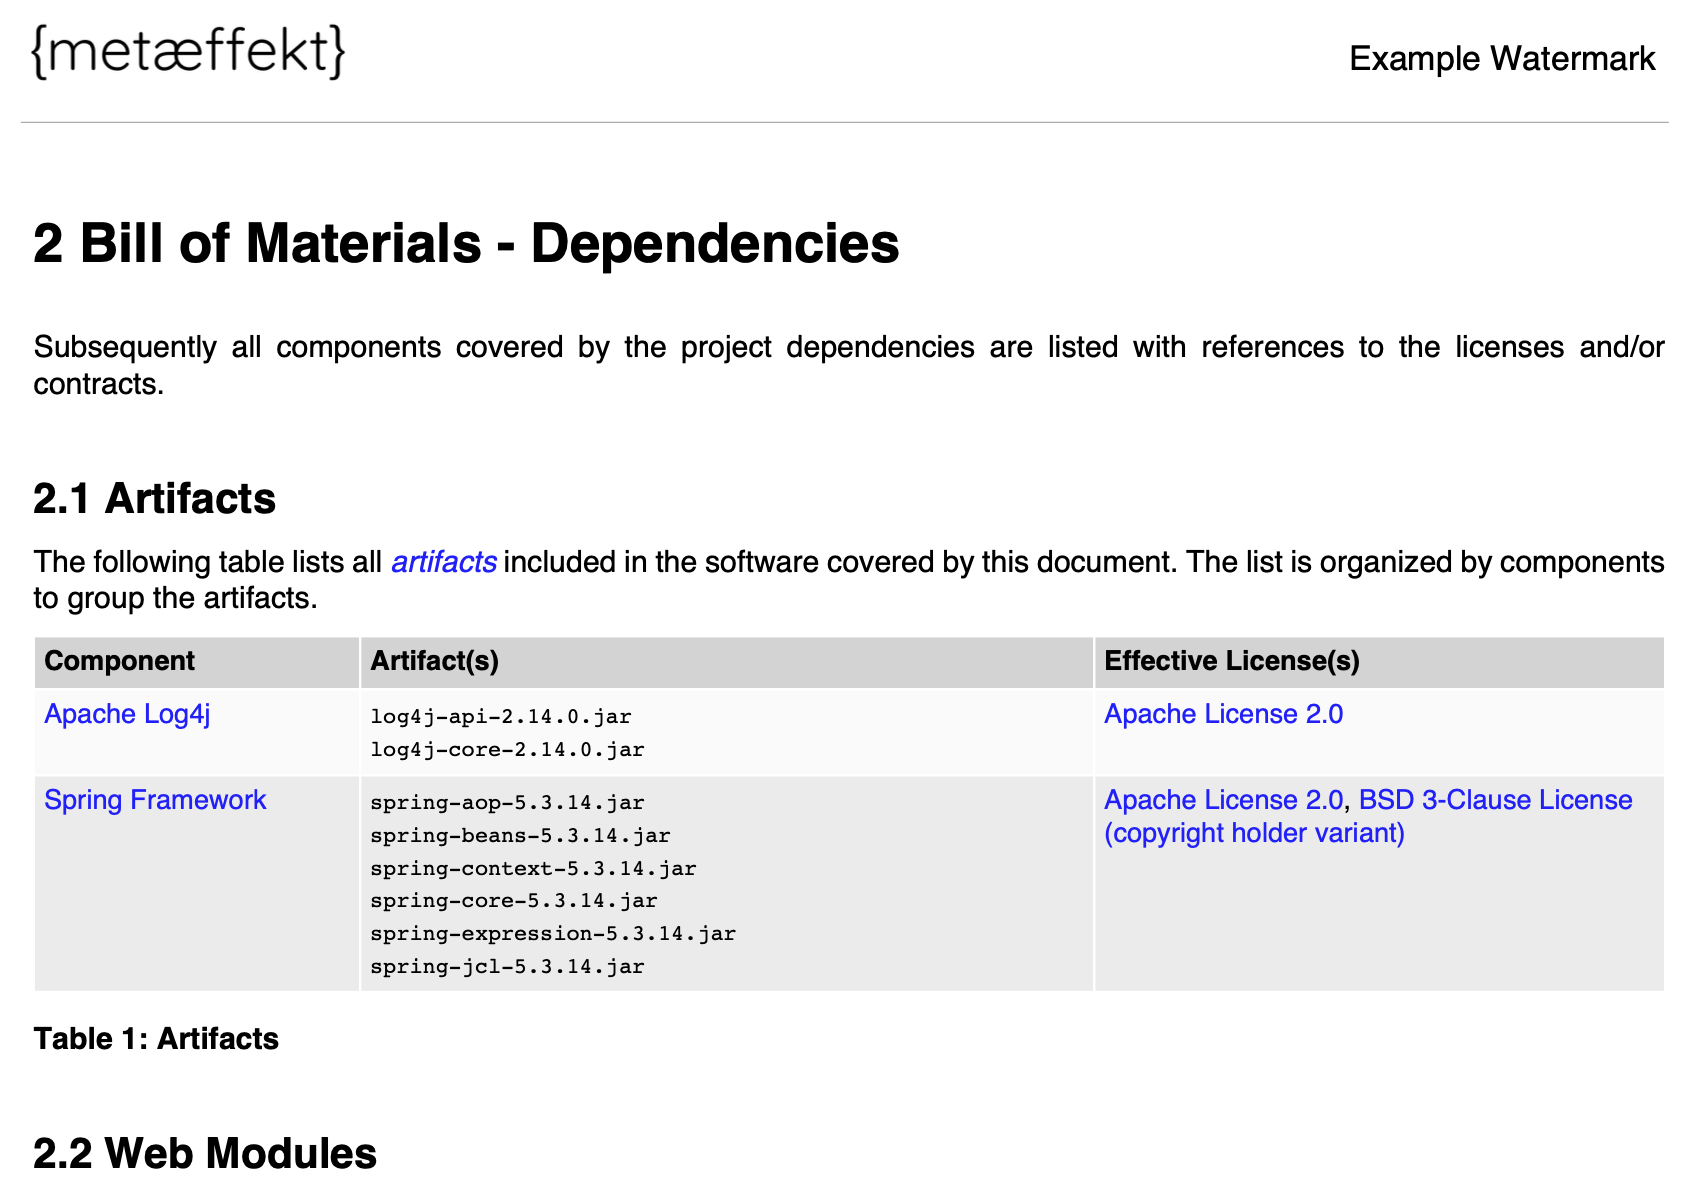
\includegraphics[width=\textwidth]{einleitung/screenshot-annex-01.png}
    \caption{Ausschnitt aus einem beispielhaften Software-Annex, der die tabellarische Aufstellung der Software-Komponenten (Component), der zugehörigen Artefakte (Artifacts) und der für sie geltenden Lizenzen (Effective Licenses) zeigt. Diese detaillierte Zuordnung ist die Grundlage für die rechtssichere Auslieferung von Software.}
    \label{fig:annex-01}
\end{figure}

Den im Annex dokumentierten Copyright-Statements kommt ebenfalls eine wesentliche Bedeutung zu.
Ihre korrekte und unveränderte Wiedergabe ist in vielen Fällen Teil der rechtlichen Verpflichtungen, die sich aus den jeweiligen Lizenzen ergeben.
Abbildung~\ref{fig:annex-02} illustriert diesen Sachverhalt am Beispiel der Komponente \textit{Spring Framework}.
Dort wird explizit aufgeführt, dass die BSD 3-Clause Lizenz die Reproduktion des spezifischen Copyright-Vermerks \enquote{Copyright (c) 2000-2011 INRIA, France Telecom All rights reserved.} erfordert.
Die Extraktion solcher Vermerke ist daher keine technische Formalität, sondern eine Notwendigkeit zur Lizenzerfüllung.
Die Vollständigkeit und Fehlerfreiheit dieser Informationen wirkt sich somit direkt auf die Rechtskonformität des gesamten Softwareprodukts aus.
Die automatisierte und präzise Identifikation dieser Statements ist eine Voraussetzung für ein effektives und skalierbares License Compliance Management.

\begin{figure}[ht]
    \centering
    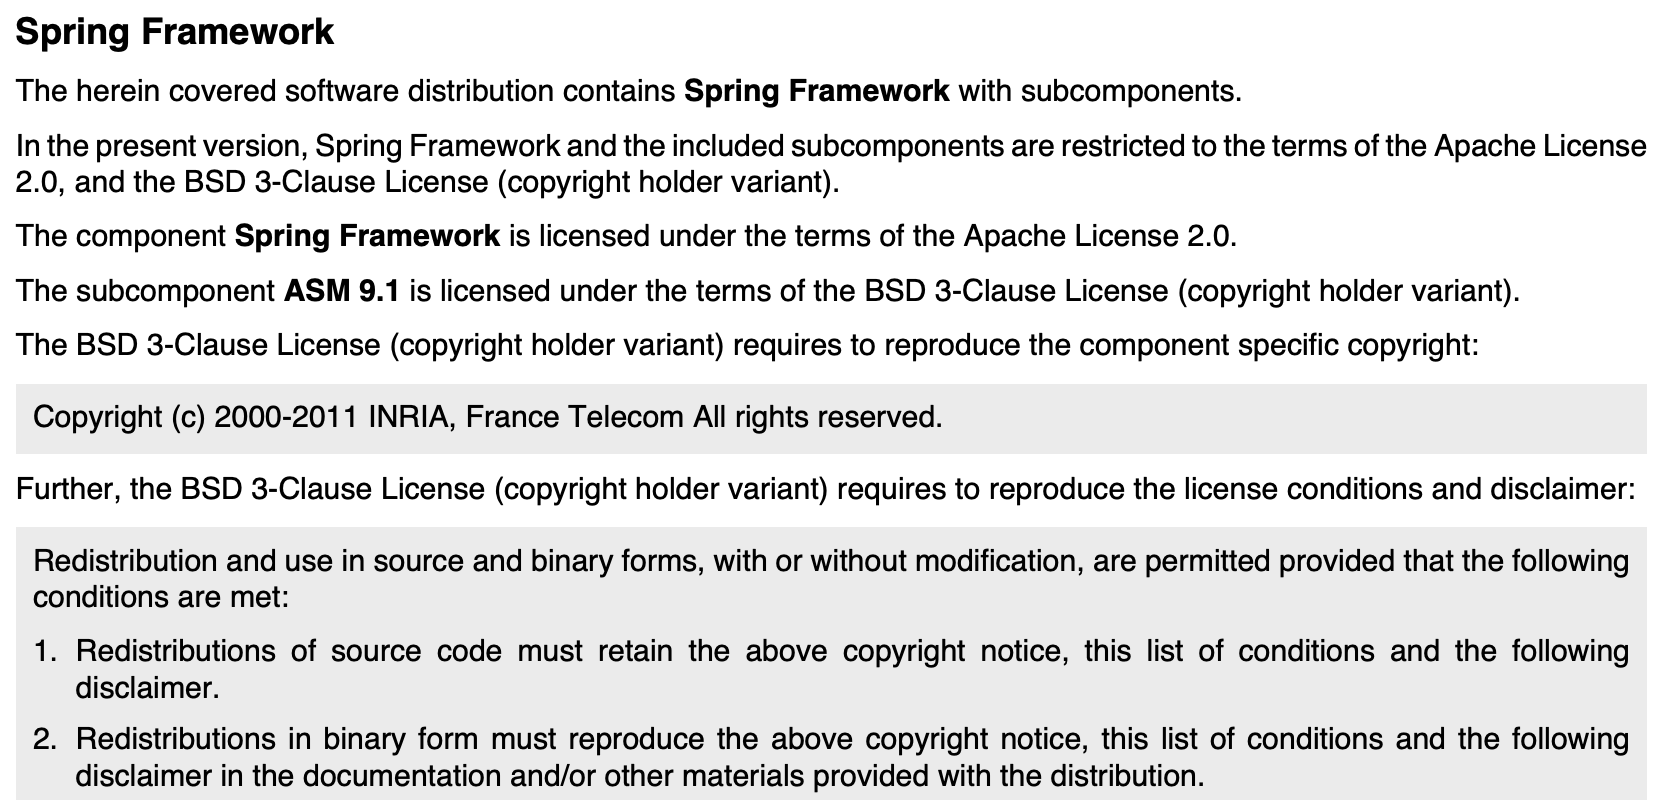
\includegraphics[width=\textwidth]{einleitung/screenshot-annex-02.png}
    \caption{Beispielhafter Auszug aus dem Abschnitt \textit{License Notices} eines Annex. Es wird gezeigt, wie für die Komponente \textit{Spring Framework} eine konkrete Lizenzverpflichtung der BSD 3-Clause Lizenz erfüllt wird, indem der dazugehörige Copyright-Vermerk sowie die Lizenzbedingungen exakt reproduziert werden.}
    \label{fig:annex-02}
\end{figure}

% ======================================================================================================================

\section{Darstellung der Problemstellung bei der automatisierten Extraktion von Copyright-Informationen}\label{sec:problemstellung}

Die automatisierte Extraktion von Copyright-Informationen ist für die rechtssichere Nutzung von Software unerlässlich, doch die etablierten Werkzeuge stoßen in der Praxis an grundlegende methodische Grenzen.
Die größte Herausforderung besteht darin, dass urheberrechtliche Vermerke in Softwareprojekten keinem einheitlichen Standard folgen, sondern über Jahrzehnte in unzähligen Variationen und oft formlos direkt im Quellcode oder begleitenden Hinweisen eingebracht wurden.
Bestehende Analysesysteme setzen vorwiegend auf starre, regelbasierte Verfahren, die dieser Vielfalt nicht gerecht werden und die oft subtilen, kontextabhängigen Bedeutungen nicht erfassen können.

Diese technologische Limitierung führt zu mehreren Problemen.
Zum einen verändern die Werkzeuge häufig die extrahierten Copyright-Vermerke, indem sie beispielsweise Formatierungen oder die ursprüngliche Schreibweise anpassen.
Solche Eingriffe können jedoch die Integrität und die rechtliche Aussagekraft der Originalangabe verfälschen.
Zum anderen scheitern diese Systeme oft daran, zusammengehörige Blöcke mit mehreren Copyright-Angaben als eine Einheit zu erkennen, was zum Verlust des erforderlichen Kontextes führt.
Darüber hinaus ist die Erkennung aller beitragenden Autoren unzureichend, da viele Mitwirkende an Positionen im Quellcode genannt werden, die von einfachen Suchmustern nicht erfasst werden.

Das Kernproblem resultiert folglich aus der methodischen Diskrepanz zwischen deterministischen, regelbasierten Extraktionsansätzen und der heterogenen, semantisch vielfältigen Natur der zu analysierenden Daten.
Die daraus folgenden fehlerhaften und unvollständigen Extraktionen erfordern einen hohen manuellen Nachbesserungsaufwand und stellen ein fortwährendes Risiko für die Lizenz-Compliance dar.

% ======================================================================================================================

\section{Zielsetzung der Arbeit}\label{sec:zielsetzung}

Das zentrale Ziel dieser Arbeit ist die Entwicklung und Bewertung eines neuartigen, auf künstlicher Intelligenz basierenden Copyright-Scanners.
Dieser soll die methodischen Schwächen existierender, regelbasierter Systeme adressieren.
Die Untersuchung konzentriert sich darauf, wie \glspl{llm} genutzt werden können, um Copyright-Informationen präziser und im Einklang mit spezifischen Compliance-Richtlinien zu extrahieren.
Es wird ein Prototyp implementiert und evaluiert, um das Potenzial dieses Ansatzes für den praktischen Einsatz im Lizenzmanagement aufzuzeigen.

% ======================================================================================================================

\section{Abgrenzung des Projektumfangs und Erläuterung der methodischen Vorgehensweise}\label{sec:abgrenzung}

Diese Arbeit grenzt sich insofern von verwandten Forschungsfeldern ab, als dass sie nicht die Aufdeckung von Copyright-Verstößen zum Ziel hat.
Der Projektumfang konzentriert sich stattdessen vollständig auf die Entwicklung und Bewertung von Methoden zur präzisen Extraktion der urheberrechtlich relevanten Metadaten.
Die methodische Vorgehensweise ist mehrstufig aufgebaut und folgt einem iterativen Ansatz, bei dem die Erkenntnisse aus den einzelnen Phasen direkt in die kontinuierliche Verbesserung und Anpassung einer im Rahmen dieser Arbeit entwickelten Policy einfließen.

Zuerst erfolgt eine systematische Datenaggregation, um eine hochwertige Test- und Evaluationsgrundlage zu schaffen.
Darauf aufbauend wird ein umfassender Benchmark verschiedener Sprachmodelle durchgeführt, um ein geeignetes Basismodell zu identifizieren.
Im nächsten Schritt wird dessen Leistung durch gezieltes Prompt-Engineering iterativ verbessert.
Abschließend wird mittels Fine-Tuning untersucht, ob ein spezialisiertes, kleineres Modell eine vergleichbare Genauigkeit bei höherer Effizienz erreichen kann.